
\chapter{Implementation}

In this chapter we shall outline which builds specified in the design were implemented, and examine how they were done so with detailed reference to the methods and technologies used. 

\section{Resources Used}
To aid development, we utilised several existing solutions as bases for our implementations. In particular:
\begin{itemize}
    \item \textbf{Google's Sample WebTransport Client} \cite{wt_js_client_sample} was used as the basis for our WebTransport builds' client code. This code implements a basic event log, provides several functions for sending and receiving both datagrams and stream data and establishes the WebTransport connection. 
    \item \textbf{web-platform-test's WebTransport-compatible QUIC-enabled python server} \cite{web-platform-tests} was used as the basis for our WebTransport builds' server code. web-platform-test is a test suite that allows developers to run several automated tests on their servers to ensure they are robust and capable - we do not utilise these tests, but we do make use of the provided server. This code handles all the basic server logic.
    \item \textbf{Web Dev Simplified} \cite{web_dev_simplified} provided a video tutorial on how to set up a WebRTC video conferencing application. This was used to develop our WebRTC build and was not significantly further built upon.
\end{itemize}
\hfill{} \\
We shall now examine how our WebTransport builds were implemented.

\section{WebTransport}

Our WebTransport builds meet our previously defined "must have" requirements - we have a build that sends and receives video data via datagrams and one that does the same via streams. However, the builds do not meet any of our "should have" requirements. Firstly, due to time constraints, they do not send or receive audio or text data. Secondly, the datagrams build does actually support multiple users in one session, but is not optimised to do so. Finally, the streams build does not support multiple users in one session at all - this was because of the way packet headers are sent via streams, which we shall discuss later in the paper. 

% \begin{figure}[h]
%     \centering
%     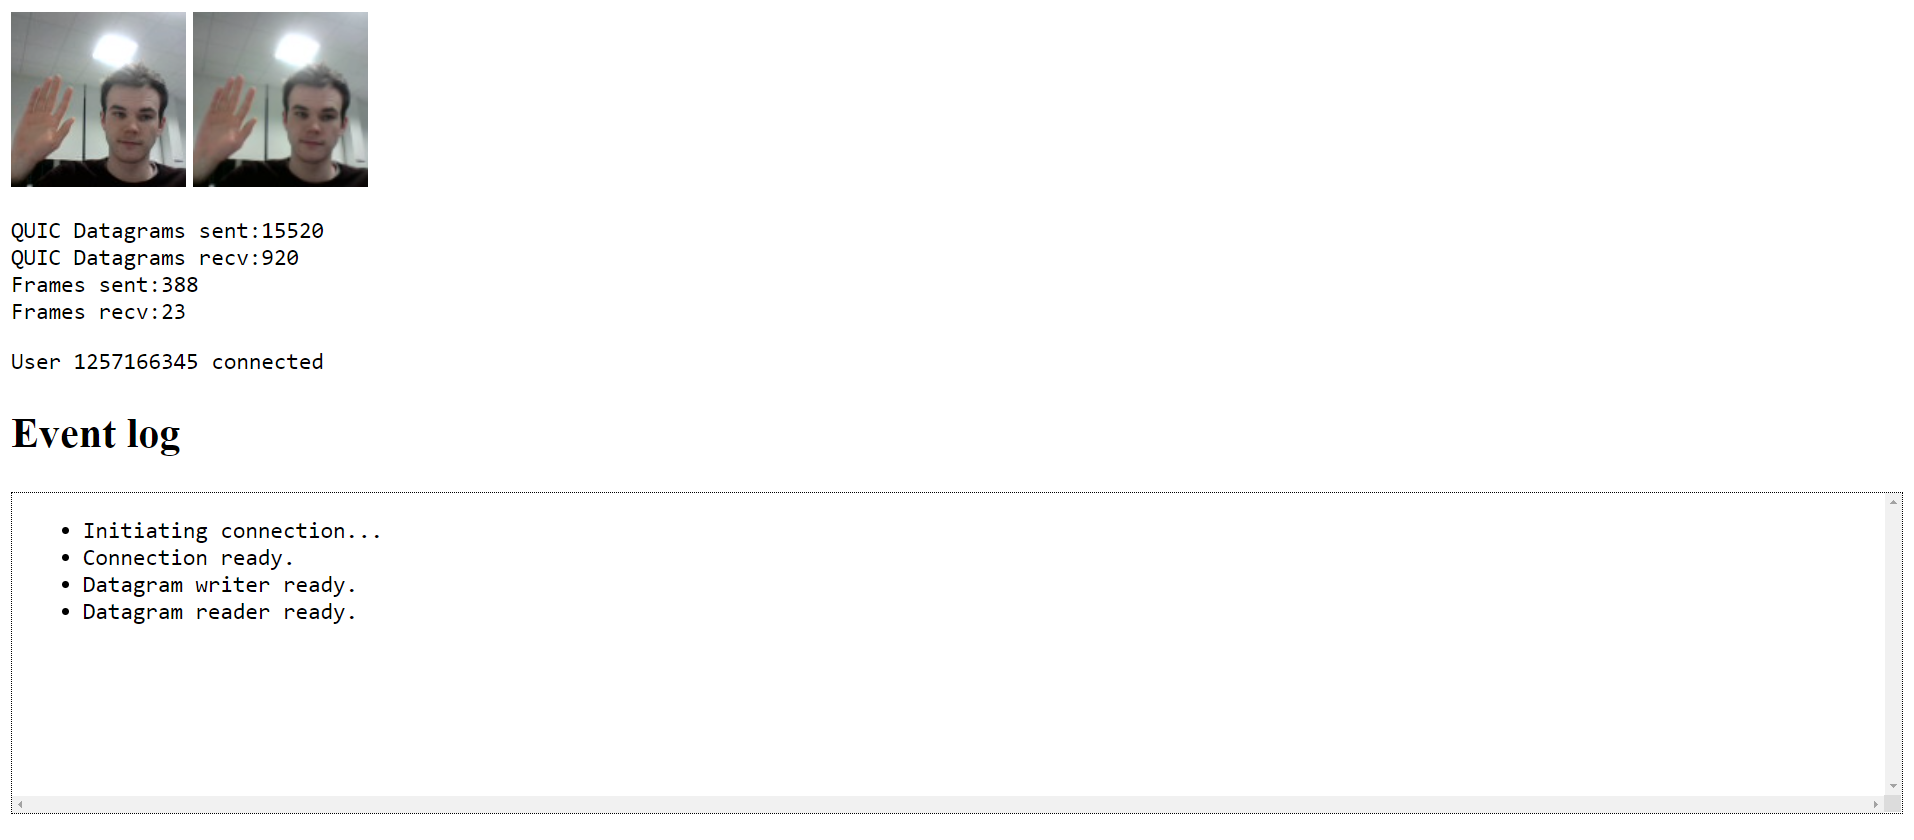
\includegraphics[width=0.95\linewidth]{images/webtransport build.png}
% 	\caption{A screenshot of the WebTransport build.}
%     \label{wt_build_screenshot}
% \end{figure}

The final design of the WebTransport builds is close to the initial wireframe (as seen in Figure \ref{wireframe}), albeit without the chat log (as this was not implemented). Additionally, the high-level system operation is consistent with the system diagram given in our Design chapter, specifically illustrated in Figure \ref{wt_systemdiagram}.

In this section, we shall first examine the shared functionality between the two builds. The server used by the two builds is actually the same, so we shall start with discussing this and how it supports both datagrams and streams. Following this, we shall examine our two WebTransport clients - one for the Datagrams build, and one for the Streams build. Again, there is some shared functionality here, so this shall be examined before diverging into build-specific functionality.

\subsection{WebTransport Server}
The base server provided by web-platform-tests is effective, yet limited. It is a WebTransport over HTTP/3 server written in python - it utilises the aioquic library \cite{aioquic} to implement QUIC and WebTransport functionality. It is capable of establishing a connection, receiving data via datagrams or streams and sending that data back to the original sender. As it is capable of handling both datagrams and streams data, we use this as the basis for both our Datagrams and Streams WebTransport builds.

Our expansion added the functionality to send received data to other existing connections. It did so by keeping a list of session objects and sending data to each session object that was not the sender's own session.

\begin{lstlisting}[language=python, caption={Added server functionality of sending data to other existing connections (streams example).}, label=lst:callahan]
    ...
    
    session = WebTransportSession(self, counter, request_headers)
    connections.append(session)
        
    ...
    
    for connection in connections:
        if connection != self._session:
            if (self._session.stream_is_unidirectional(stream_id)):
                pass
            else:
                connection.send_stream_data(stream_id, data, stream_ended)                    
                self._run_callback("stream_data_received", stream_id, data, stream_ended)

\end{lstlisting}
    
Another significant expansion was the ability for the server to read the packet headers sent to it. This was tailored for my client implementation and so worked with DataViews and 32-bit unsigned integers (this will be explained further in the paper). The function worked by putting the received data into a DataView class defined in python and then decoding the contents to extract multiple 32-bit unsigned integer at various byte offsets. These integers corresponded to the packet's headers. This code can be seen in Listing \ref{lst:server-decode-headers}. Ultimately, this feature was not utilised in any of our final builds. However, in future, it could be useful for implementing specific server logic in WebTransport applications - for example, in a scenario where connection becomes unstable, the server could receive some header indicating that it should send received data back utilising streams instead of datagrams to ensure reliability over timeliness. Furthermore, it is useful for logging and testing purposes.

\subsection{WebTransport Clients}

We shall now examine how the WebTransport clients operate and what shared functionality there is between the Datagrams and Streams builds. The two builds send data in similar fashion but receive data slightly differently, so we shall explain the sending process of both builds before diverging to talk about the two receiving processes.
\hfill\\
\subsubsection{Sending Data - Datagrams and Streams Builds}
\hfill\\
After establishing the connection to the server, the client immediately requests the video data from the user's camera and generates a unique user ID. Then, the client sends single frames of video data at a regular arbitrary interval by repeatedly calling the \textit{sendData} function - we found that 100ms worked suitably (resulting in an output of 10 frames per second) and used this for our evaluations later. This was an arbitrarily chosen value. 

\textit{sendData} works by utilising a while loop; this loop continues to send data until a variable, \textit{offset}, is found to be greater than the length of the image data. This works in two stages.

Firstly, at the start of every loop, the \textit{size} variable is used to signify the size of the sent packet. We chose \textit{size} to have a value of 1004 as our headers take up 20 bytes, and we decided to have our packets be 1024 bytes long (this was an arbitrarily selected value). Then, the following \textit{if} statement checks if \textit{offset} in addition to \textit{size} is greater than the length of the image data. If it is, \textit{size} is decreased to only send the required amount of image data to complete a full frame. A representation of this process can be seen in Figure \ref{wt_sending_trimchunk}, and the code that alters \textit{size} is seen in Listing \ref{lst:resize}.

\begin{figure}[h]
    \centering
    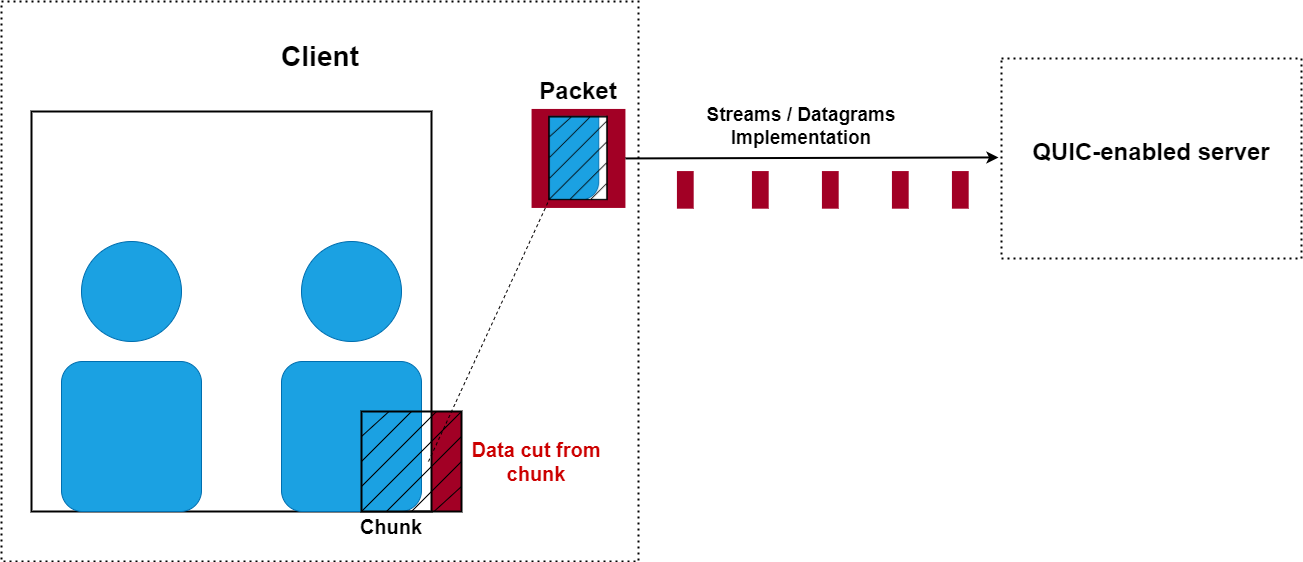
\includegraphics[width=0.95\linewidth]{images/cutting chunk sending.png}
	\caption{The WebTransport client resizing sent chunk to only send what is necessary to complete a frame.}
    \label{wt_sending_trimchunk}
\end{figure}

\hfill{} \\

\begin{lstlisting}[language=javascript, caption={First part of functionality that exits loop when full frame is sent.}, label=lst:resize]
    let size = 1004;
        if (offset + size > imgData.data.length) {
            size = imgData.data.length - offset;
    }

\end{lstlisting}

The second stage is at the end of the loop; here, after a chunk of data is sent, the client adds the \textit{size} of the sent chunk and checks if \textit{offset} is now greater than the length of the image data. If so, this indicates that the full frame is sent, the loop is exited and the client moves on to sending the next frame.  This is seen in Listing \ref{lst:second_stage}.

\begin{lstlisting}[language=javascript, caption={Second part of functionality that exits loop when full frame is sent.}, label=lst:second_stage]
    offset += size;
    if (offset >= imgData.data.length) { 
        break;
    }
\end{lstlisting}

Now, we shall examine how each chunk is encoded and sent. A chunk is encoded by slicing the image data between the current \textit{offset} and the succeeding amount of data according to \textit{size}. An illustration of this can be seen in Figure \ref{wt_sending_chunkoffset}.

\begin{figure}[h]
    \centering
    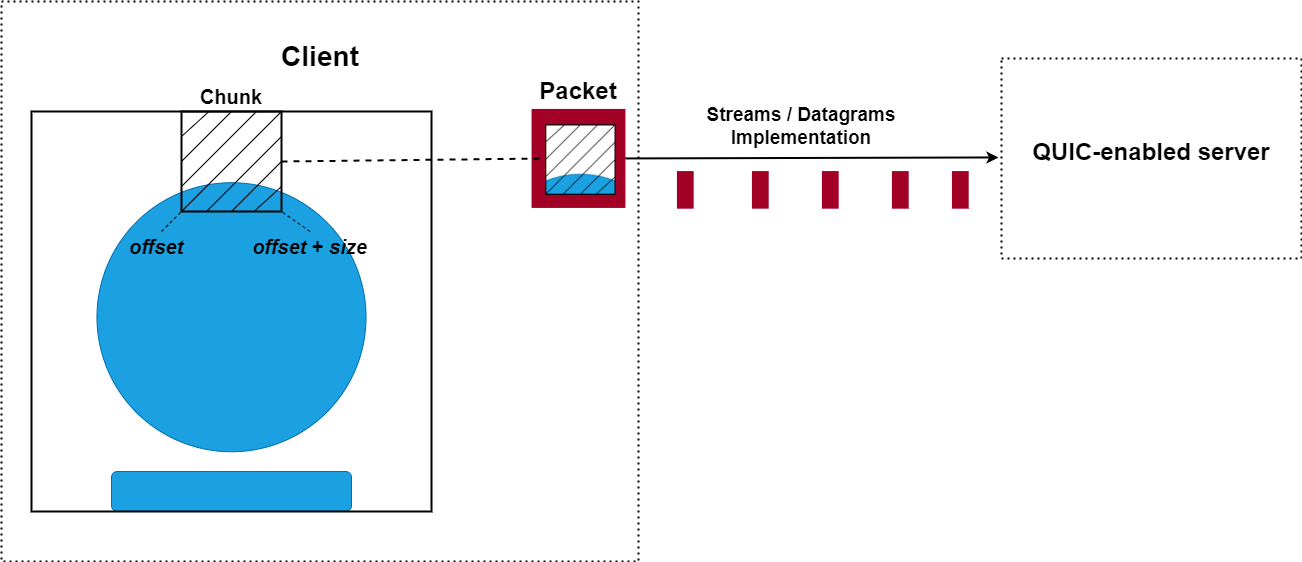
\includegraphics[width=0.95\linewidth]{images/how chunk is selected.png}
	\caption{The WebTransport client selecting a chunk of data to process.}
    \label{wt_sending_chunkoffset}
\end{figure}

Then, a buffer \textit{writeBuffer} is created. This buffer is an \textit{ArrayBuffer} and is stored within a \textit{Uint8ClampedArray} - this array is the length of a predefined header size (\textit{HEADERSIZE}) in addition to the value of \textit{size}. We use a \textit{Uint8ClampedArray} simply because our received image data is stored in a \textit{ImageData} object, whcih also utilises a \textit{Uint8ClampedArray}.

Then, this buffer is put into a \textit{DataView}. We use the \textit{DataView} here as an API of sorts to access the bytes at different arbitrary byte-positions; this is useful as we insert and extract headers for later processing. For the Datagrams build, we insert our headers into the first 20 bytes of the packet. Our headers are \textit{streamId} (the predefined unique user ID), \textit{sequenceNumber} (the sequence number of the packet within the frame), \textit{eof} (a boolean indication of whether the frame has been fully sent), \textit{frameNumber} and \textit{ts} (a timestamp of when the packet was sent from WebTransport). The packet is then sent, thus concluding our data transmission algorithm. 

\begin{lstlisting}[language=javascript, caption={The encoding and transmission of our video data.}, label=lst:callahan]
    const chunk = imgData.data.slice(offset, offset + size);

    let writeBuffer = new Uint8ClampedArray(HEADERSIZE + chunk.length);
    const dv = new DataView(writeBuffer.buffer, 0);

    writeBuffer.set(chunk, HEADERSIZE);
    
    sequenceNumber++;

    dv.setUint32(0, streamId);
    dv.setUint32(4, sequenceNumber);  
    dv.setUint32(8, offset + size >= imgData.data.length ? 1 : 0); // eof
    dv.setUint32(12, frameNumber);
    dv.setUint32(16, (Date.now()/1000));

    await currentTransportDatagramWriter.write(dv); 
\end{lstlisting}

It is important to note here that we do not utilise headers in our Streams build as message boundaries are not preserved and headers are consequently useless for later processing. Although a way around this may be explored in future, there is no reasonable way to extract these headers within the scope of this project.

We shall now examine how each build receives data. The two builds are essentially the same, but the Datagrams build has added functionality to handle packet reordering and loss. Because of this, we shall examine the shared functionality between the two before discussing the Datagrams build's unique features.
\hfill\\
\subsubsection{Receiving Data - Datagrams and Streams Builds}
\hfill\\
The client receives data as often as it can, reading data as soon as it is available in a while loop that only exits when the connection is closed. 

If a new \textit{streamId} is detected, the client generates a new video feed and renders all incoming data in this feed. One distinction here is that the Datagrams build reads the unique \textit{streamId} from the packet headers, whereas the Streams build just defines this itself as either "1" or "2" - this is why the Streams build is incapable of handling more than two users in one session. 

A dictionary, \textit{connections}, is used to track each user session - each dictionary contains an associated \textit{buffer} and \textit{bufferOffset}. 

These are all the similarities between the two builds. We shall now discuss the builds separately.
\hfill\\
\subsubsection{Receiving Data - Streams Build:}
\hfill\\
We shall refer to the data inside a received packet as \textit{value} from here on. Similarly to before with \textit{offset} and \textit{size} (see Figure \ref{wt_sending_chunkoffset}), we check to see if the connection's \textit{bufferOffset} in addition to the \textit{dataSize} (the size of \textit{value}) is greater than the size of the frame (\textit{FRAMESIZE)} - if it is, we amend the size of the data array we are reading and use this to update our \textit{buffer} later. This is done to ensure that we do not add more data to the generated frame than necessary. Next, the connection's \textit{buffer} has \textit{value} appended to it (sliced according to the potentially altered \textit{dataSize}) at an index of \textit{bufferOffset}. Then, \textit{bufferOffset} is increased by the value of \textit{dataSize}. The remaining data that is cut off when we sliced \textit{value} is then added to another array, \textit{leftoverData}, which we will use later. The code for this process can be seen in Listing \ref{buildingbuffer}. The purpose of all this is to "build up" the \textit{buffer} until we have all the data needed to render a full frame.

\begin{figure}[h]
    \centering
    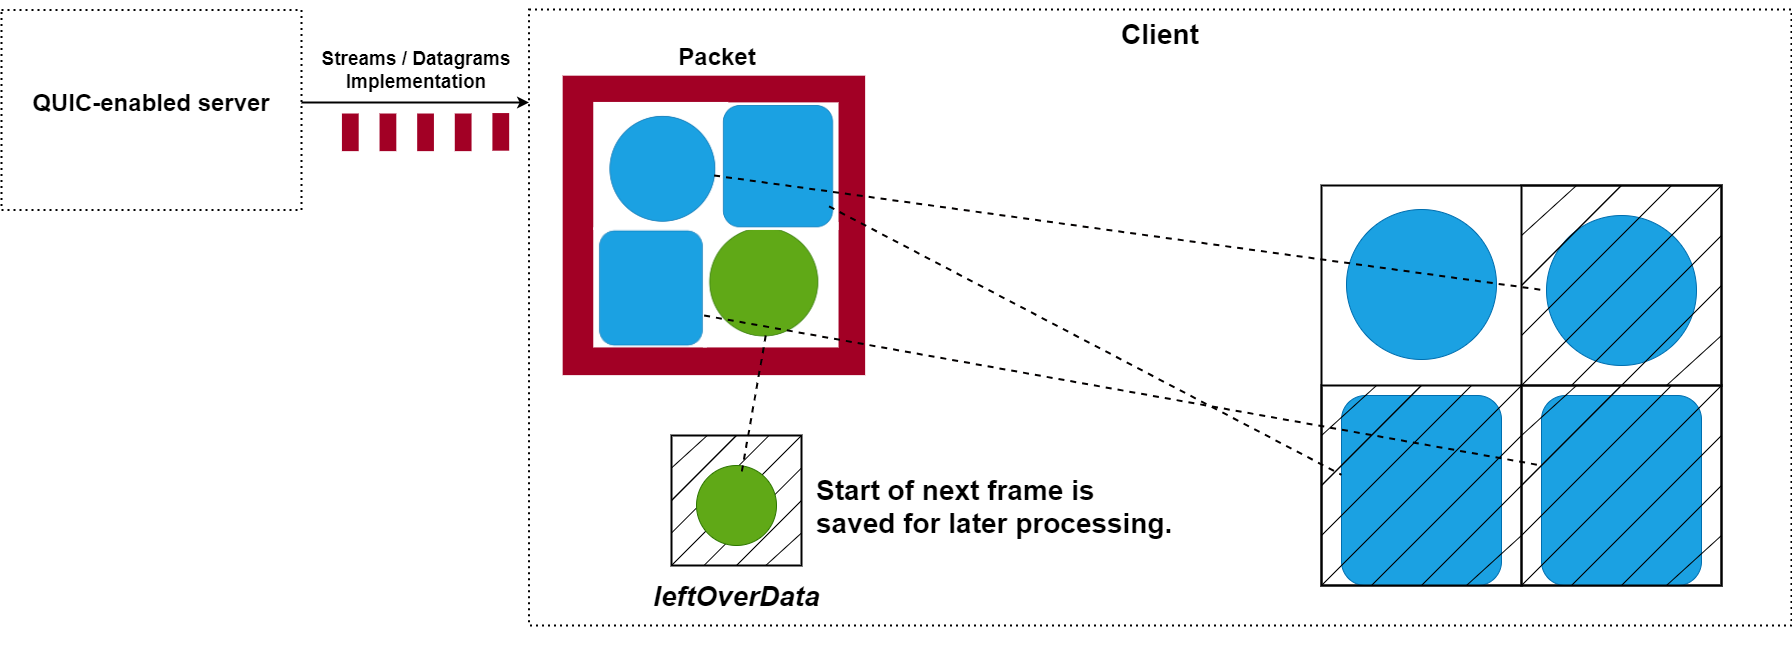
\includegraphics[width=1\linewidth]{images/wt_streams_leftoverdata.png}
	\caption{The WebTransport client building up a frame whilst working without message boundaries (streams).}
    \label{wt_streams_leftoverdata}
\end{figure}

\begin{lstlisting}[language=javascript, caption={Streams build's client building up the buffer.}, label=buildingbuffer]
    if (connections[streamId].bufferOffset + dataSize > FRAMESIZE) {
      dataSize = FRAMESIZE - connections[streamId].bufferOffset; 
    }
    connections[streamId].buffer.set(value.slice(0, dataSize), connections[streamId].bufferOffset);
    connections[streamId].bufferOffset += dataSize;

    leftoverData = value.slice(dataSize, );
\end{lstlisting}

\textit{leftoverData} is necessary as, once again, streams do not preserve message boundaries. Consequently, chunks sent from the other client are encapsulated arbitrarily into packets, meaning that a chunk does not arrive in the exact packet it is sent in; this is illustrated in Figure \ref{wt_streams_leftoverdata}. This results in some packets containing data from parts of multiple chunks, meaning we must employ additional parsing of received packets. 

Next, we will check if \textit{bufferOffset} is equal to \textit{FRAMESIZE}; if it is, we have all the data necessary to comprise a full frame and so the frame is rendered. Once the frame is rendered, \textit{bufferOffset} is reset.

Finally, if this occurs and there is some data in \textit{leftoverData}, we essentially redo the process of Listing  \ref{buildingbuffer} - this ensures that no data is wasted and the next frame does not have any data missing from the start of its \textit{buffer}. Then, \textit{leftoverData} is reset and the process begins again.

The client for the Streams build was far easier to implement than the Datagrams build counterpart.
\hfill\\
\subsubsection{Receiving Data - Datagrams Build}
\hfill\\
The Datagrams build's client has the same general process of adjusting \textit{bufferOffset} and \textit{buffer} depending on \textit{dataSize} and rendering when the end of the frame is reached. Regarding the latter point, this is done via the \textit{eof} header; furthermore, the rest of the headers are used throughout the client (unlike with the Streams build). In particular, the Datagrams build is capable of hosting multiple connections as it is able to render new video feeds based on the unique \textit{streamId} header by creating a new video feed and \textit{connection} dictionary whenever a new unique \textit{streamId} is detected.

We shall now examine the main feature of the Datagrams build that sets it apart: the techniques that handle packet loss and disorder. 

The client handles packets arriving in a disordered fashion by creating a queue - this queue is a dictionary of arrays with each key corresponding to a frame number and each value storing an array containing the relevant packets. This dictionary shall be referred to as \textit{dict}. A new key/value pair is created every time a new \textit{frameNumber} is detected. As new datagrams come in, if the \textit{value} (i.e. the payload data from a datagram) is not present in the dictionary (i.e it is not a duplicate datagram) and the \textit{frameNumber} has not been discarded (more on this later), the \textit{value} is added to the queue. The queue is constantly maintained in an ascending order by sorting the keys every time a new \textit{value} is added. Next, to actually process the datagrams in order, the client attempts to take the first \textit{value} from the lowest present \textit{frameNumber}. If it succeeds, the datagram shall be handled as normal until \textit{eof} is received - once the frame has been completed, the \textit{frameNumber} is deleted as a key value from \textit{dict}, the frame is rendered and the process restarts. This process is very similar to the one outlined in Figure \ref{wt_design_latepackets}.

However, what if the frame is not completed and there are no datagram \textit{value}s in the queue for the lowest \textit{frameNumber}? This may occur when packets, notably one containing the \textit{eof} header, are lost. To combat this, the client implements an arbitrary timeout on each \textit{frameNumber} - this is set to 10 retries. If the client attempts to read these missing datagrams 10 times and none arrive, the \textit{frameNumber} is discarded from the queue and added to an array of discarded frames, \textit{forgottenFrames} - this array is used in the earlier \textit{if} statement to discard datagrams that correspond to these "timed out" frames. The code for this process can be seen in Listing \ref{lst:discarding_frames}.

\begin{lstlisting}[language=javascript, caption={Datagrams build's client handling timed out frames.}, label=lst:discarding_frames]
    value = dict[keys[0]].shift();
    if (!value) {
      counter++;
      if (counter == 10) {
        forgottenFrames.push(prevFrameNumber)
        render(connections[streamId], frameNumber);
        delete dict[keys[0]];
        counter = 0;
        prevSequenceNumber = 1;
      }
      continue;
    }
\end{lstlisting}

The client also handles packets that go missing during the construction of a frame (i.e. in the scenario where the start and end of the frame still arrive). It does this by keeping track of a variable, \textit{prevSequenceNumber} in addition to the header variable \textit{sequenceNumber2} (note that it is named \textit{sequenceNumber2} at this point as this is the header of the dequeued packet rather than the originally received packet). If the client detects that \textit{prevSequenceNumber} is not equal to one less than \textit{sequenceNumber2} (and on the condition that it is not the first datagram in the frame), \textit{bufferOffset} will be altered to "skip past" the gaps left by the missing packets. This results in a slight glitch in the rendered frame's appearance as the missing parts of the frame will display as those parts from the previous frame - this is because \textit{buffer} is not erased, but instead overwritten, and so the previous data is preserved. This process is the same as that depicted in Figure \ref{wt_design_shifteddata}. 

\begin{lstlisting}[language=javascript, caption={Datagrams build's client handling lost datagrams.}, label=lst:callahan]
    if (prevSequenceNumber != (sequenceNumber2 - 1) && sequenceNumber2 != 1) {
      connections[streamId2].bufferOffset = (connections[streamId2].bufferOffset + dataSize*(sequenceNumber2-prevSequenceNumber)-dataSize);
    }
\end{lstlisting}

This concludes the notable elements of the WebTransport implementations. Both WebTransport implementations combined took approximately 117 hours to complete, taking into account time spent designing, researching, configuring Chrome and scrapping features.

%============================================================================================================================

% \subsection{Build 1: Datagrams}

% \subsubsection{The Server}

% \subsubsection{The Client}

% %============================================================================================================================

% \subsection{Build 2: Streams}

% \subsubsection{The Server}

% \subsubsection{The Client}

% %============================================================================================================================

\section{WebRTC}
We implemented a WebRTC video conferencing application by following an online tutorial from "Web Dev Simplified" \cite{web_dev_simplified} that utilises WebRTC in conjunction with PeerJS and socket.io; this took us roughly 2 hours to develop a working build. This build met all of its design specifications except for a chat function, which was dropped due to time constraints. Additionally, this build met two of the specified "should have" requirements: "A WebRTC build that sends and receives video data" and "All builds should send and receive audio data". As this build is not my own implementation, we shall only include details that we feel are necessary to better understand the upcoming evaluation rather than discussing technical accomplishments at length.

\subsection{socket.io and Rooms}
socket.io is a JavaScript library that enables real-time, bi-directional communication between web clients and servers. socket.io utilises WebSockets - this is an established API that allows for reliable, ordered and untimely data transfer between a client and a server in a single stream. WebSockets is similar to WebTransport, but is not as customisable, suffers from head-of-line blocking and transports data via TCP rather than QUIC \cite{websockets_mozilla_docs}, thus making it generally unsuitable for media transfer.

In our application, we utilised socket.io to facilitate the communications relating to setting up "rooms" for users to join. These rooms are again based on a unique ID generated by the application. In the following code, a unique ID is generated when a user starts the application and this ID is appended to the URL the user is connected to.

\begin{lstlisting}[language=javascript, caption={A unique ID is generated and added to the user's connected URL.}, label=lst:callahan]
    app.get('/', (req, res) => {
        res.redirect(`/${uuidV4()}`)
    })
\end{lstlisting}

This URL is passed to the frontend of the code so that users can share their room ID.

socket.io communicates with a simple server set up utilising Express, a Node.js web application framework; this server is exclusively utilised for logic relating to rooms. Several event listeners are established in both the frontend and backend of the application, and we utilise these listeners and corresponding "emitters" to undertake actions. For example, when the user loads the application, the frontend emits a "join-room" event - a listener in the server receives this message and broadcasts a "user-connected" message to the other users stating that a certain user ID has connected. Another listener in the frontend receives this message and runs a function to connect to this user ID. 

\begin{lstlisting}[language=javascript, caption={socket.io facilitated communications.}, label=lst:callahan]
    ... (frontend code) ...
    socket.emit('join-room', ROOM_ID, id)
    
    ...(backend code) ...
    socket.on('join-room', (roomId, userId) => {
        ...
        socket.broadcast.to(roomId).emit('user-connected', userId)
        
    ... (frontend code) ...
    socket.on('user-connected', userId => {
        connectToNewUser(userId, stream)
    })
\end{lstlisting}

All of this communication is facilitated through socket.io. Additionally, it is used to handle user disconnection.

We shall now examine how PeerJS is used when this \textit{connectToNewUser} function is called.

\subsection{PeerJS, Connection Establishment and Sending/Receiving Data}
PeerJS is a JavaScript library that, from a developer's perspective, greatly simplifies WebRTC's connection establishment process - PeerJS allows developers to create a peer-to-peer media stream connection utilising nothing but a unique ID.  In the application, we generate another unique ID (\textit{userId}) to connect to our peer.

PeerJS utilises a "peer server" to act as a connection broker. As soon as the user launches the application, we have them connect to this peer server. Since both users will be communicating everything regarding connection establishment via this peer server, PeerJS is used to create event listeners and emitters in just the frontend. 
After socket.io gets users in the same room and calls \textit{connectToNewUser}, we utilise PeerJS in this function to establish a connection to our peer and transmit data. We create \textit{myPeer}, a PeerJS object that represents a peer. \textit{connectToNewUser} uses PeerJS' \textit{call} function to "call" the other peer and transmit our media stream via WebRTC's media channel. Then, the function listens to the event "stream" that takes in the peer's media stream and appends it to the frontend video grid.

\begin{lstlisting}[language=javascript, caption={Connection establishment and data transmission via PeerJS and WebRTC.}, label=lst:callahan]
    function connectToNewUser(userId, stream) {
        const call = myPeer.call(userId, stream)
        const video = document.createElement('video')
        call.on('stream', userVideoStream => {
            addVideoStream(video, userVideoStream)
        })
    ...
\end{lstlisting}

The client code also has a listener that responds to this call and sends back its own media stream, also via PeerJS and WebRTC's media channel.

\begin{lstlisting}[language=javascript, caption={Responding to the connection establishment, receiving media data and transmitting media data back via WebRTC.}, label=lst:callahan]
    myPeer.on('call', call => {
        call.answer(stream)
        const video = document.createElement('video')
        call.on('stream', userVideoStream => {
            addVideoStream(video, userVideoStream)
        })
    })
\end{lstlisting}

In addition to this, socket.io handles further connection-related logic such as peer disconnections.  

This build illustrates how simple it is from a developer's perspective to send and receive live media data. Unlike the WebTransport builds, the main complexity in this code relates to session and connection establishment rather than the handling of transmitted and received data, and even then the functionality is mostly handled by our additional libraries (socket.io and PeerJS). 

With this, we have our three builds ready for evaluation. 


% What did you do to implement this idea, and what technical achievements did you make?
% \section{Guidance}
% You can't talk about everything. Cover the high level first, then cover important, relevant or impressive details.

% \section{General guidance for technical writing}

% These points apply to the whole dissertation, not just this chapter.

% \subsection{Figures}
% \emph{Always} refer to figures included, like Figure \ref{fig:relu}, in the body of the text. Include full, explanatory captions and make sure the figures look good on the page.
% You may include multiple figures in one float, as in Figure \ref{fig:synthetic}, using \texttt{subcaption}, which is enabled in the template.


% % Figures are important. Use them well.
% \begin{figure}[h]
%     \centering
%     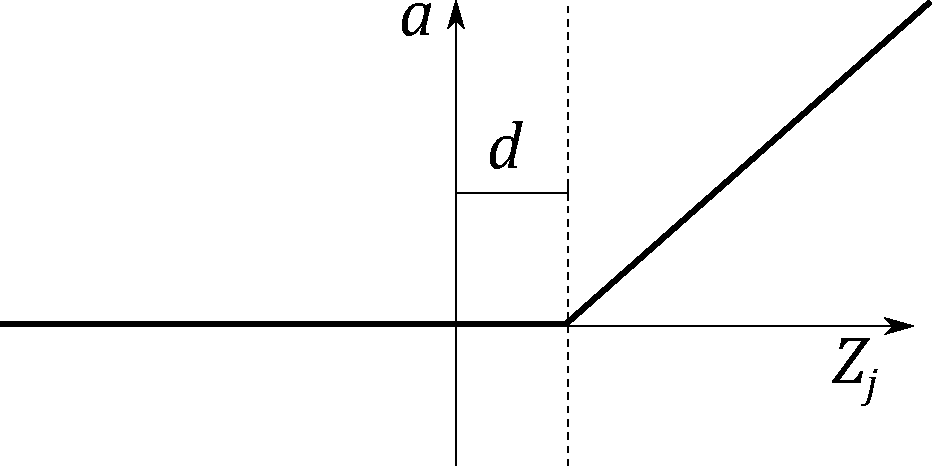
\includegraphics[width=0.5\linewidth]{images/relu.pdf}    

%     \caption{In figure captions, explain what the reader is looking at: ``A schematic of the rectifying linear unit, where $a$ is the output amplitude,
%     $d$ is a configurable dead-zone, and $Z_j$ is the input signal'', as well as why the reader is looking at this: 
%     ``It is notable that there is no activation \emph{at all} below 0, which explains our initial results.'' 
%     \textbf{Use vector image formats (.pdf) where possible}. Size figures appropriately, and do not make them over-large or too small to read.
%     }

%     % use the notation fig:name to cross reference a figure
%     \label{fig:relu} 
% \end{figure}


% \begin{figure}[h] 
%     \centering
%     \begin{subfigure}[b]{0.45\textwidth}
%         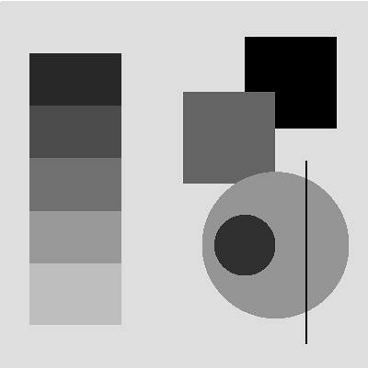
\includegraphics[width=\textwidth]{images/synthetic.png}
%         \caption{Synthetic image, black on white.}
%         \label{fig:syn1}
%     \end{subfigure}
%     ~ %add desired spacing between images, e. g. ~, \quad, \qquad, \hfill etc. 
%       %(or a blank line to force the subfigure onto a new line)
%     \begin{subfigure}[b]{0.45\textwidth}
%         
\includegraphics[width=\textwidth]{images/synthetic_2.png}
%         \caption{Synthetic image, white on black.}
%         \label{fig:syn2}
%     \end{subfigure}
%     ~ %add desired spacing between images, e. g. ~, \quad, \qquad, \hfill etc. 
%     %(or a blank line to force the subfigure onto a new line)    
%     \caption{Synthetic test images for edge detection algorithms. \subref{fig:syn1} shows various gray levels that require an adaptive algorithm. \subref{fig:syn2}
%     shows more challenging edge detection tests that have crossing lines. Fusing these into full segments typically requires algorithms like the Hough transform.
%     This is an example of using subfigures, with \texttt{subref}s in the caption.
%     }\label{fig:synthetic}
% \end{figure}

% \clearpage

% \subsection{Equations}

% Equations should be typeset correctly and precisely. Make sure you get parenthesis sizing correct, and punctuate equations correctly 
% (the comma is important and goes \textit{inside} the equation block). Explain any symbols used clearly if not defined earlier. 

% For example, we might define:
% \begin{equation}
%     \hat{f}(\xi) = \frac{1}{2}\left[ \int_{-\infty}^{\infty} f(x) e^{2\pi i x \xi} \right],
% \end{equation}    
% where $\hat{f}(\xi)$ is the Fourier transform of the time domain signal $f(x)$.

% \subsection{Algorithms}
% Algorithms can be set using \texttt{algorithm2e}, as in Algorithm \ref{alg:metropolis}.

% % NOTE: line ends are denoted by \; in algorithm2e
% \begin{algorithm}
%     \DontPrintSemicolon
%     \KwData{$f_X(x)$, a probability density function returing the density at $x$.\; $\sigma$ a standard deviation specifying the spread of the proposal distribution.\;
%     $x_0$, an initial starting condition.}
%     \KwResult{$s=[x_1, x_2, \dots, x_n]$, $n$ samples approximately drawn from a distribution with PDF $f_X(x)$.}
%     \Begin{
%         $s \longleftarrow []$\;
%         $p \longleftarrow f_X(x)$\;
%         $i \longleftarrow 0$\;
%         \While{$i < n$}
%         {
%             $x^\prime \longleftarrow \mathcal{N}(x, \sigma^2)$\;
%             $p^\prime \longleftarrow f_X(x^\prime)$\;
%             $a \longleftarrow \frac{p^\prime}{p}$\;
%             $r \longleftarrow U(0,1)$\;
%             \If{$r<a$}
%             {
%                 $x \longleftarrow x^\prime$\;
%                 $p \longleftarrow f_X(x)$\;
%                 $i \longleftarrow i+1$\;
%                 append $x$ to $s$\;
%             }
%         }
%     }
    
% \caption{The Metropolis-Hastings MCMC algorithm for drawing samples from arbitrary probability distributions, 
% specialised for normal proposal distributions $q(x^\prime|x) = \mathcal{N}(x, \sigma^2)$. The symmetry of the normal distribution means the acceptance rule takes the simplified form.}\label{alg:metropolis}
% \end{algorithm}

% \subsection{Tables}

% If you need to include tables, like Table \ref{tab:operators}, use a tool like https://www.tablesgenerator.com/ to generate the table as it is
% extremely tedious otherwise. 

% \begin{table}[]
%     \caption{The standard table of operators in Python, along with their functional equivalents from the \texttt{operator} package. Note that table
%     captions go above the table, not below. Do not add additional rules/lines to tables. }\label{tab:operators}
%     %\tt 
%     \rowcolors{2}{}{gray!3}
%     \begin{tabular}{@{}lll@{}}
%     %\toprule
%     \textbf{Operation}    & \textbf{Syntax}                & \textbf{Function}                            \\ %\midrule % optional rule for header
%     Addition              & \texttt{a + b}                          & \texttt{add(a, b)}                                    \\
%     Concatenation         & \texttt{seq1 + seq2}                    & \texttt{concat(seq1, seq2)}                           \\
%     Containment Test      & \texttt{obj in seq}                     & \texttt{contains(seq, obj)}                           \\
%     Division              & \texttt{a / b}                          & \texttt{div(a, b) }  \\
%     Division              & \texttt{a / b}                          & \texttt{truediv(a, b) } \\
%     Division              & \texttt{a // b}                         & \texttt{floordiv(a, b)}                               \\
%     Bitwise And           & \texttt{a \& b}                         & \texttt{and\_(a, b)}                                  \\
%     Bitwise Exclusive Or  & \texttt{a \textasciicircum b}           & \texttt{xor(a, b)}                                    \\
%     Bitwise Inversion     & \texttt{$\sim$a}                        & \texttt{invert(a)}                                    \\
%     Bitwise Or            & \texttt{a | b}                          & \texttt{or\_(a, b)}                                   \\
%     Exponentiation        & \texttt{a ** b}                         & \texttt{pow(a, b)}                                    \\
%     Identity              & \texttt{a is b}                         & \texttt{is\_(a, b)}                                   \\
%     Identity              & \texttt{a is not b}                     & \texttt{is\_not(a, b)}                                \\
%     Indexed Assignment    & \texttt{obj{[}k{]} = v}                 & \texttt{setitem(obj, k, v)}                           \\
%     Indexed Deletion      & \texttt{del obj{[}k{]}}                 & \texttt{delitem(obj, k)}                              \\
%     Indexing              & \texttt{obj{[}k{]}}                     & \texttt{getitem(obj, k)}                              \\
%     Left Shift            & \texttt{a \textless{}\textless b}       & \texttt{lshift(a, b)}                                 \\
%     Modulo                & \texttt{a \% b}                         & \texttt{mod(a, b)}                                    \\
%     Multiplication        & \texttt{a * b}                          & \texttt{mul(a, b)}                                    \\
%     Negation (Arithmetic) & \texttt{- a}                            & \texttt{neg(a)}                                       \\
%     Negation (Logical)    & \texttt{not a}                          & \texttt{not\_(a)}                                     \\
%     Positive              & \texttt{+ a}                            & \texttt{pos(a)}                                       \\
%     Right Shift           & \texttt{a \textgreater{}\textgreater b} & \texttt{rshift(a, b)}                                 \\
%     Sequence Repetition   & \texttt{seq * i}                        & \texttt{repeat(seq, i)}                               \\
%     Slice Assignment      & \texttt{seq{[}i:j{]} = values}          & \texttt{setitem(seq, slice(i, j), values)}            \\
%     Slice Deletion        & \texttt{del seq{[}i:j{]}}               & \texttt{delitem(seq, slice(i, j))}                    \\
%     Slicing               & \texttt{seq{[}i:j{]}}                   & \texttt{getitem(seq, slice(i, j))}                    \\
%     String Formatting     & \texttt{s \% obj}                       & \texttt{mod(s, obj)}                                  \\
%     Subtraction           & \texttt{a - b}                          & \texttt{sub(a, b)}                                    \\
%     Truth Test            & \texttt{obj}                            & \texttt{truth(obj)}                                   \\
%     Ordering              & \texttt{a \textless b}                  & \texttt{lt(a, b)}                                     \\
%     Ordering              & \texttt{a \textless{}= b}               & \texttt{le(a, b)}                                     \\
%     % \bottomrule
%     \end{tabular}
%     \end{table}
% \subsection{Code}

% Avoid putting large blocks of code in the report (more than a page in one block, for example). Use syntax highlighting if possible, as in Listing \ref{lst:callahan}.

% \begin{lstlisting}[language=python, float, caption={The algorithm for packing the $3\times 3$ outer-totalistic binary CA successor rule into a 
%     $16\times 16\times 16\times 16$ 4 bit lookup table, running an equivalent, notionally 16-state $2\times 2$ CA.}, label=lst:callahan]
%     def create_callahan_table(rule="b3s23"):
%         """Generate the lookup table for the cells."""        
%         s_table = np.zeros((16, 16, 16, 16), dtype=np.uint8)
%         birth, survive = parse_rule(rule)

%         # generate all 16 bit strings
%         for iv in range(65536):
%             bv = [(iv >> z) & 1 for z in range(16)]
%             a, b, c, d, e, f, g, h, i, j, k, l, m, n, o, p = bv

%             # compute next state of the inner 2x2
%             nw = apply_rule(f, a, b, c, e, g, i, j, k)
%             ne = apply_rule(g, b, c, d, f, h, j, k, l)
%             sw = apply_rule(j, e, f, g, i, k, m, n, o)
%             se = apply_rule(k, f, g, h, j, l, n, o, p)

%             # compute the index of this 4x4
%             nw_code = a | (b << 1) | (e << 2) | (f << 3)
%             ne_code = c | (d << 1) | (g << 2) | (h << 3)
%             sw_code = i | (j << 1) | (m << 2) | (n << 3)
%             se_code = k | (l << 1) | (o << 2) | (p << 3)

%             # compute the state for the 2x2
%             next_code = nw | (ne << 1) | (sw << 2) | (se << 3)

%             # get the 4x4 index, and write into the table
%             s_table[nw_code, ne_code, sw_code, se_code] = next_code

%         return s_table

% \end{lstlisting}

%==================================================================================================================================